%********************************************************************
% Appendix
%*******************************************************
% If problems with the headers: get headings in appendix etc. right
%\markboth{\spacedlowsmallcaps{Appendix}}{\spacedlowsmallcaps{Appendix}}
\chapter{Full list of the clusters obtained with the HMRF method}
This chapter provides a quick glance over the 33 clusters generated by the HMRF method (see Chapters, \ref{ch:HMRF} and \ref{ch:biology}) in the brain of \platy{} using the $86$ genes selected from the in-situ hybridization data generated by Raju Tomer. Each cluster is presented from an apical point of view alongside the adult eyes (red cluster) for spatial reference. On each images the 3 top scoring (see Chapter \ref{ch:biology} for an explanation of the scoring process) genes are indicated.\\

\renewcommand{\thesubfigure}{\roman{subfigure}}

\begin{figure}[bth]
        \myfloatalign
        \subfloat[Cluster 1]
        {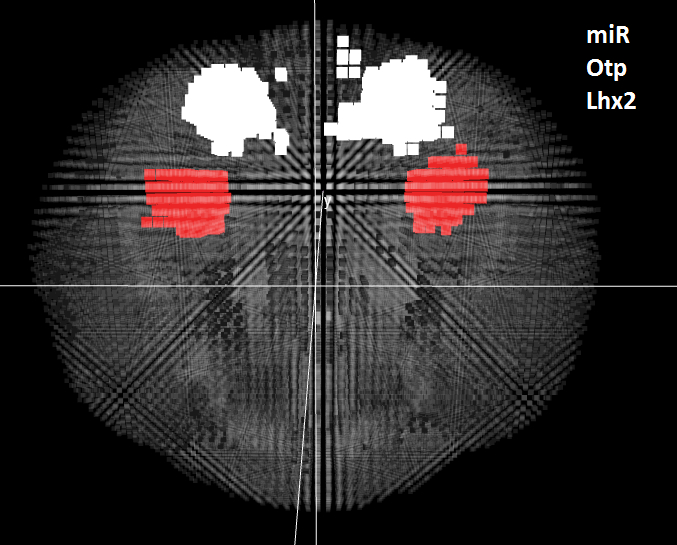
\includegraphics[width=.45\linewidth]{gfx/sup/c1.png}} \quad
        \subfloat[Cluster 2]
        {
         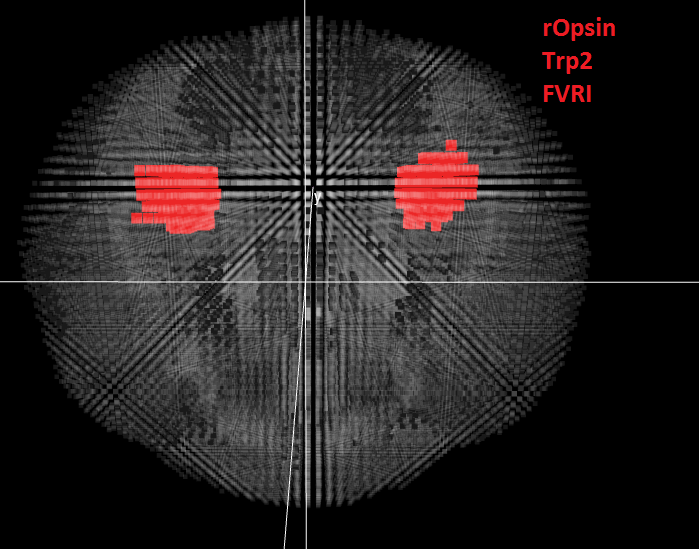
\includegraphics[width=.45\linewidth]{gfx/sup/c2.png}} \\
        \subfloat[Cluster 3]
        {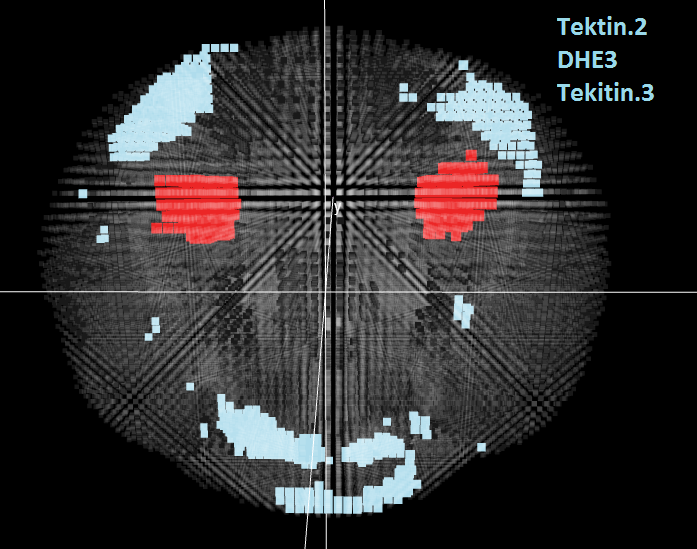
\includegraphics[width=.45\linewidth]{gfx/sup/c3.png}} \quad
        \subfloat[Cluster 4]
        {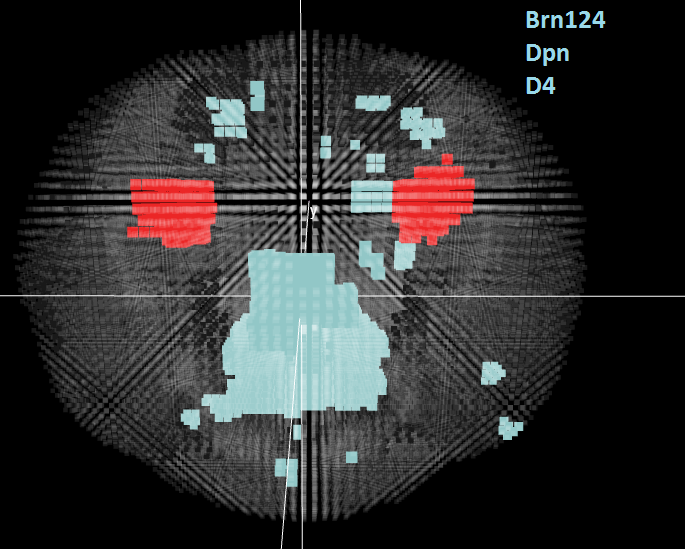
\includegraphics[width=.45\linewidth]{gfx/sup/c4.png}} \\
        \subfloat[Cluster 5]
        {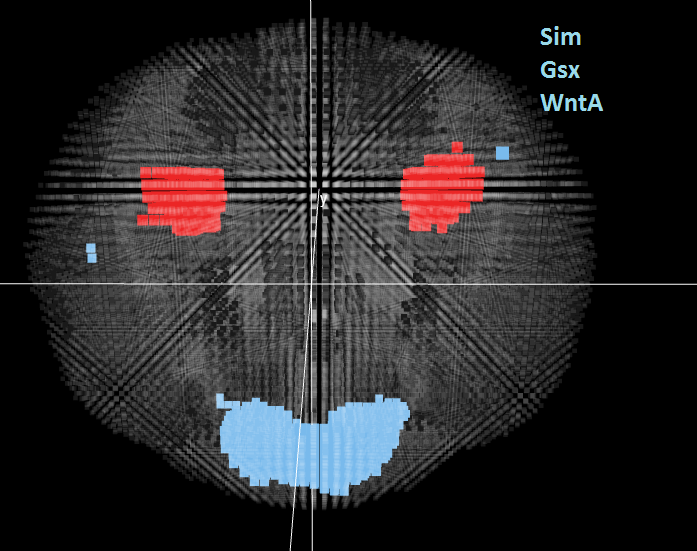
\includegraphics[width=.45\linewidth]{gfx/sup/c5.png}} \quad
        \subfloat[Cluster 6]
        {
        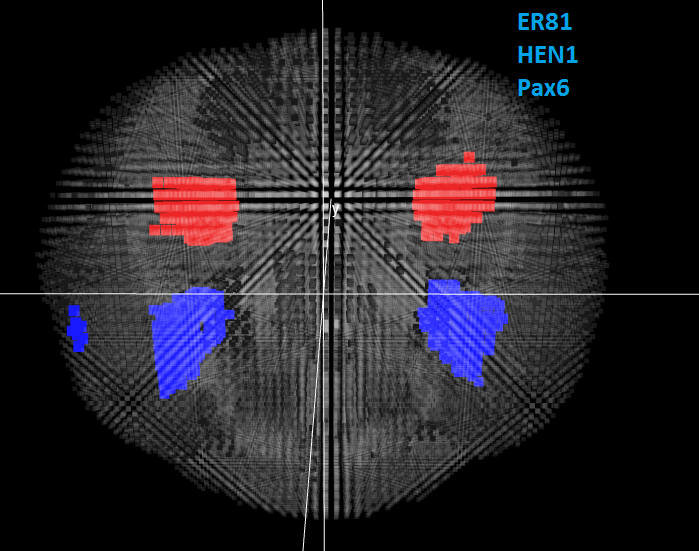
\includegraphics[width=.45\linewidth]{gfx/sup/c6.png}} \\
        \subfloat[Cluster 7]
        {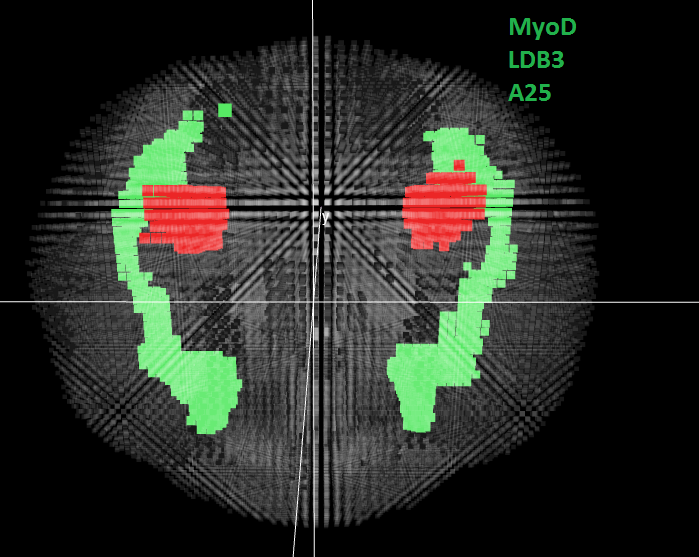
\includegraphics[width=.45\linewidth]{gfx/sup/c7.png}} \quad
        \subfloat[Cluster 8]
        {
        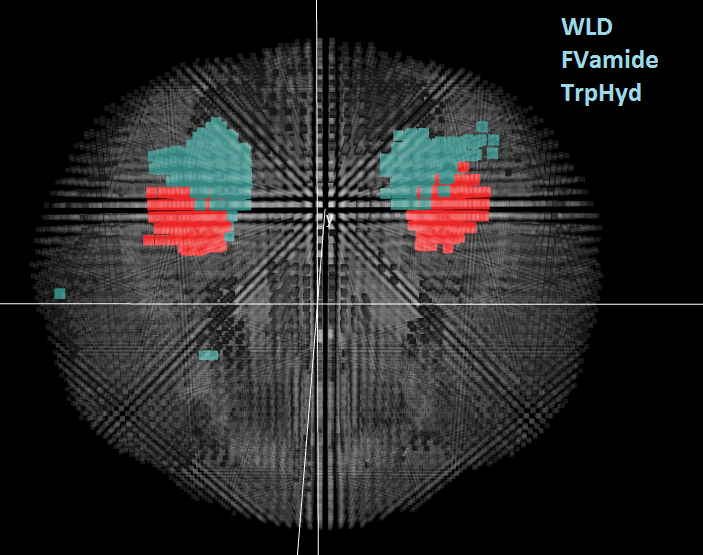
\includegraphics[width=.45\linewidth]{gfx/sup/c8.png}} \\
        \subfloat[Cluster 9]
        {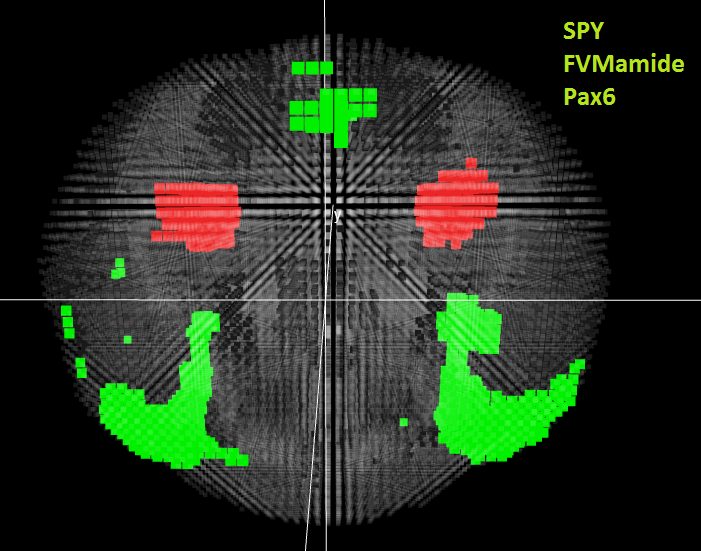
\includegraphics[width=.45\linewidth]{gfx/sup/c9.png}} \quad
        \subfloat[Cluster 10]
        {
        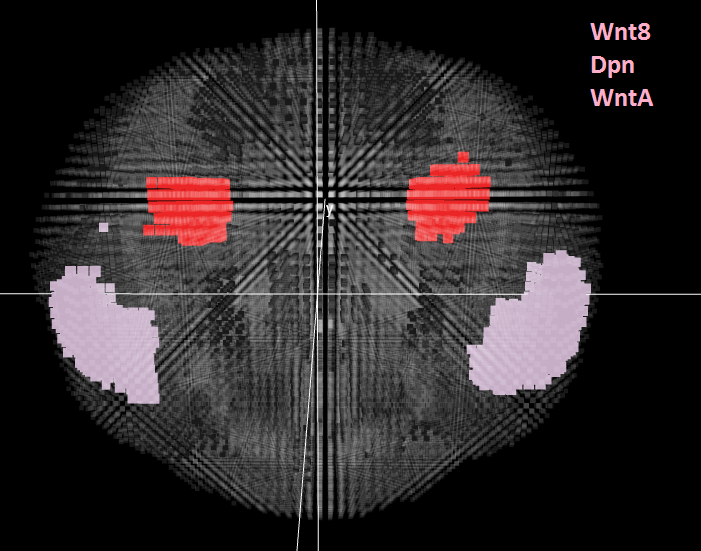
\includegraphics[width=.45\linewidth]{gfx/sup/c10.png}}
\end{figure}

\begin{figure}[bth]
         \ContinuedFloat 
        \subfloat[Cluster 11]
        {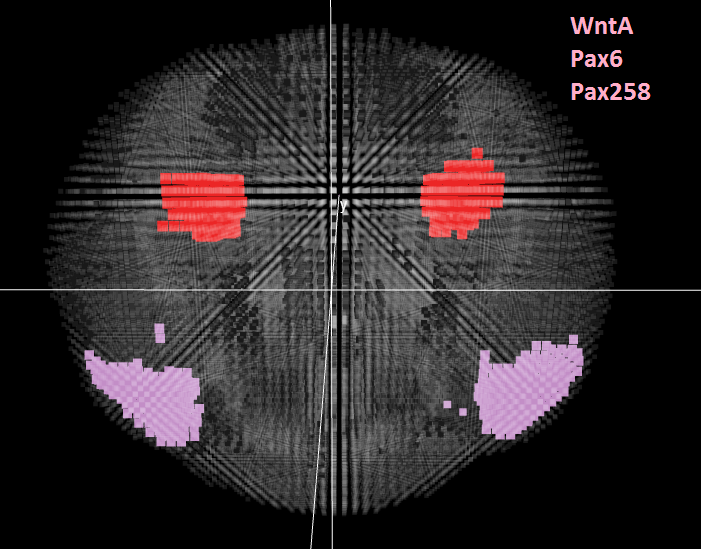
\includegraphics[width=.45\linewidth]{gfx/sup/c11.png}} \quad
        \subfloat[Cluster 12]
        {
        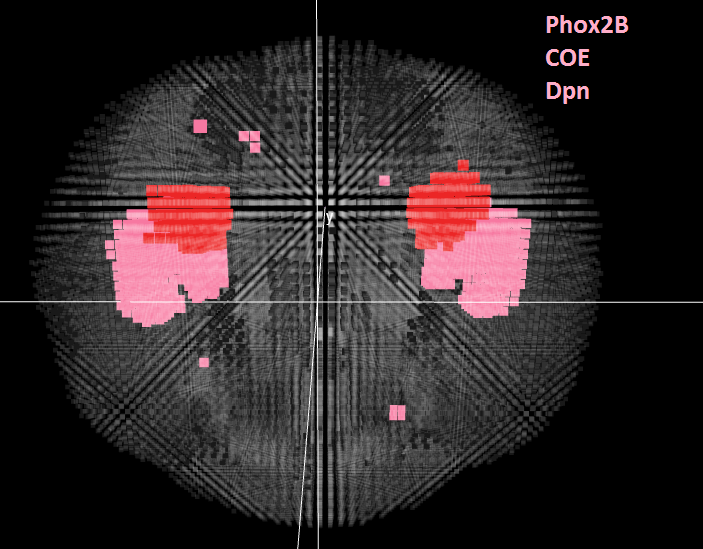
\includegraphics[width=.45\linewidth]{gfx/sup/c12.png}} \\
        \subfloat[Cluster 13]
        {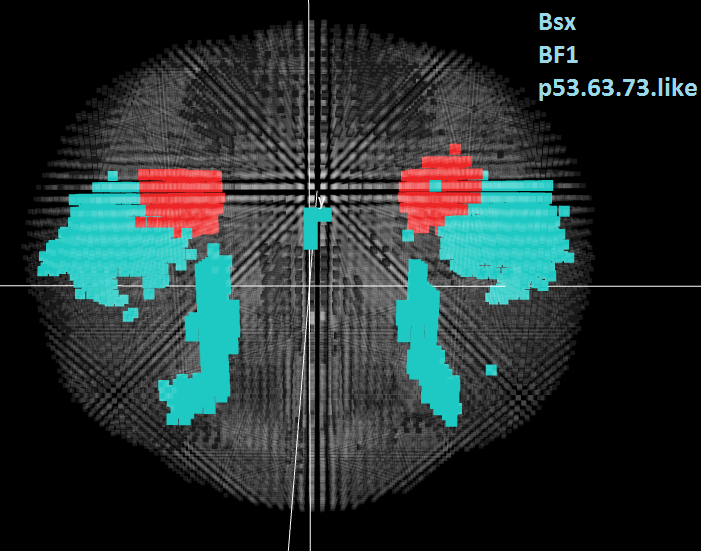
\includegraphics[width=.45\linewidth]{gfx/sup/c13.png}} \quad
        \subfloat[Cluster 14]
        {
        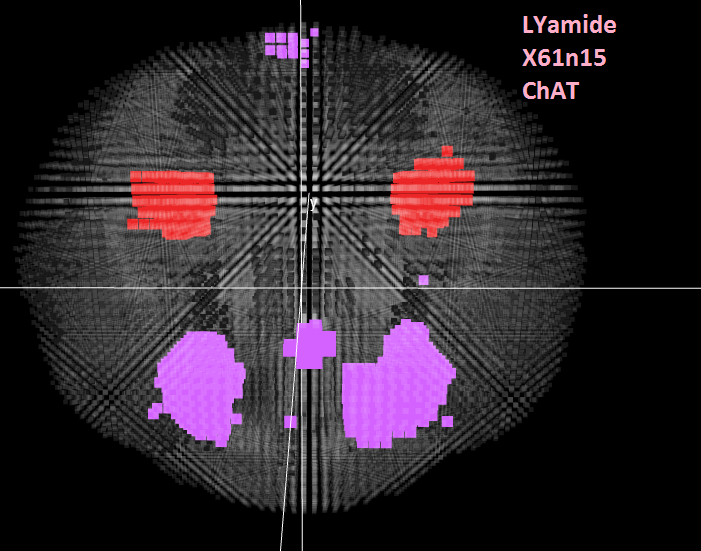
\includegraphics[width=.45\linewidth]{gfx/sup/c14.png}} \\
        \subfloat[Cluster 15]
        {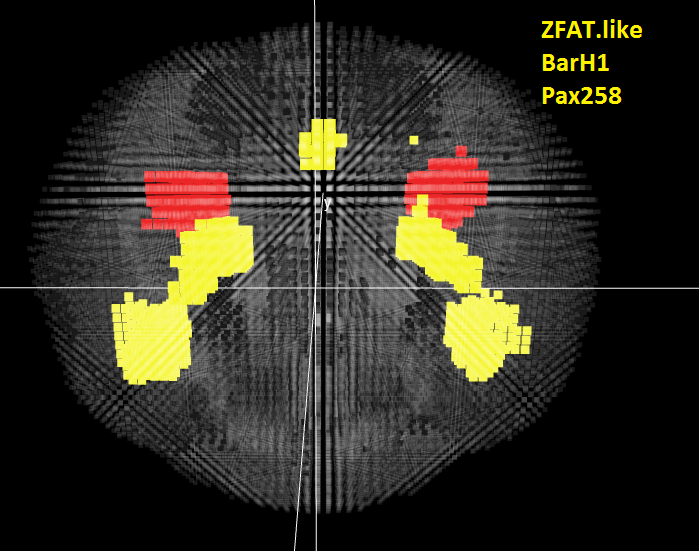
\includegraphics[width=.45\linewidth]{gfx/sup/c15.png}} \quad
        \subfloat[Cluster 16]
        {
        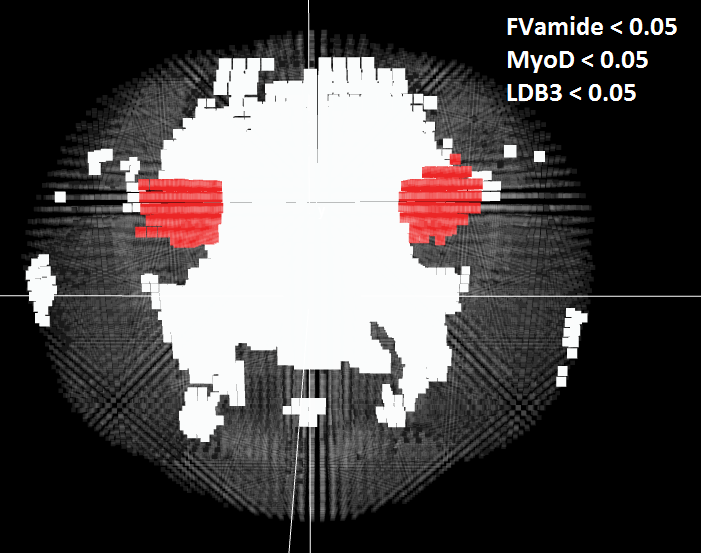
\includegraphics[width=.45\linewidth]{gfx/sup/c16.png}} \\
        \subfloat[Cluster 17]
        {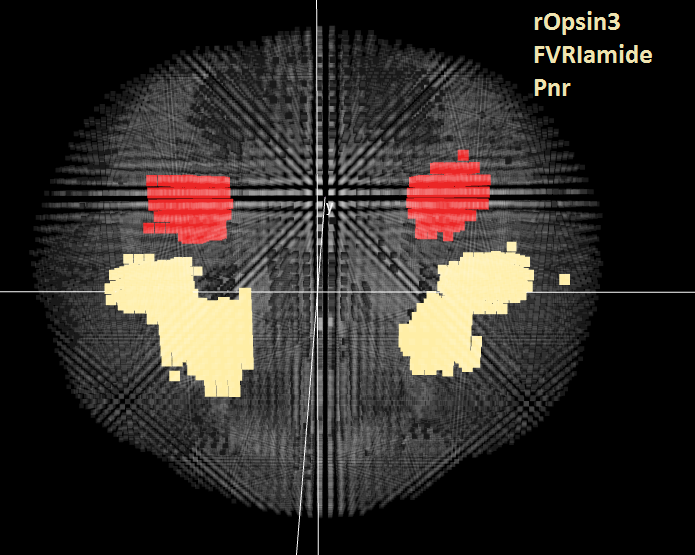
\includegraphics[width=.45\linewidth]{gfx/sup/c17.png}} \quad
        \subfloat[Cluster 18]
        {
        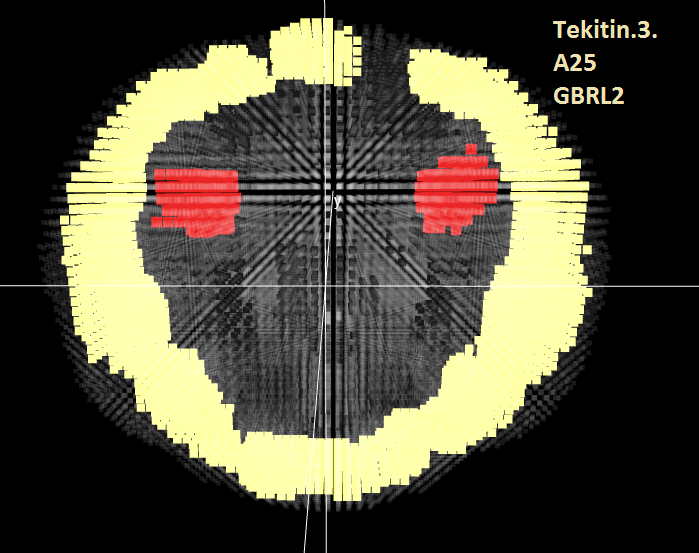
\includegraphics[width=.45\linewidth]{gfx/sup/c18.png}} \\
        \subfloat[Cluster 19]
        {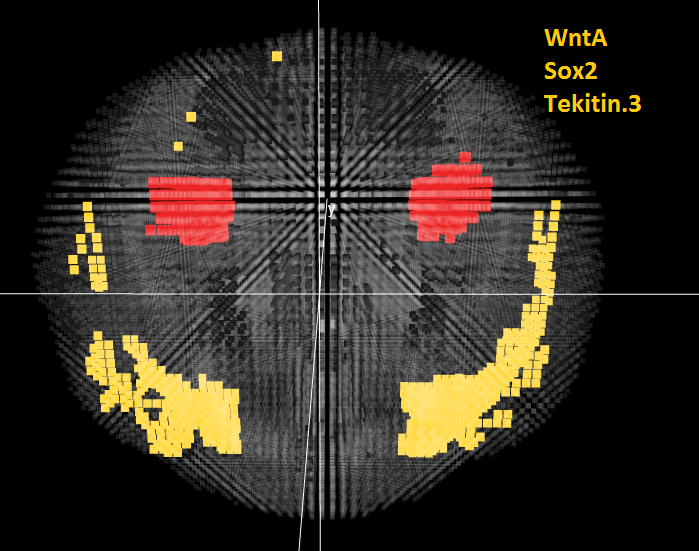
\includegraphics[width=.45\linewidth]{gfx/sup/c19.png}} \quad
        \subfloat[Cluster 20]
        {
        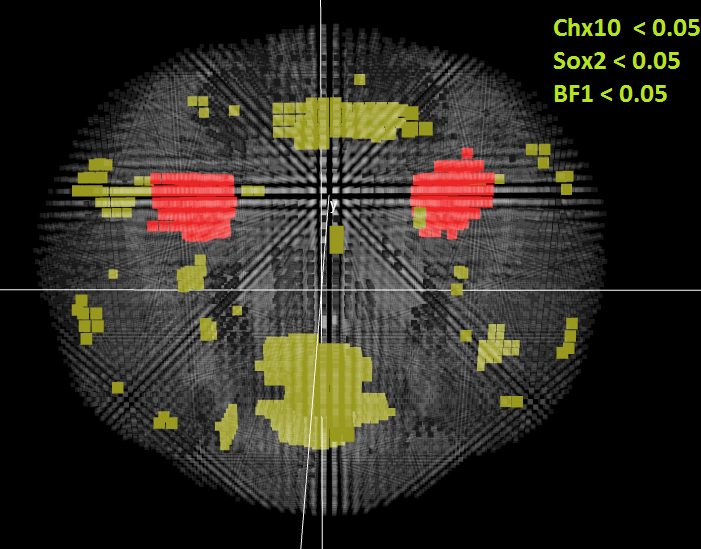
\includegraphics[width=.45\linewidth]{gfx/sup/c20.png}}
\end{figure}

\begin{figure}[bth]
       \ContinuedFloat 
        \subfloat[Cluster 21]
        {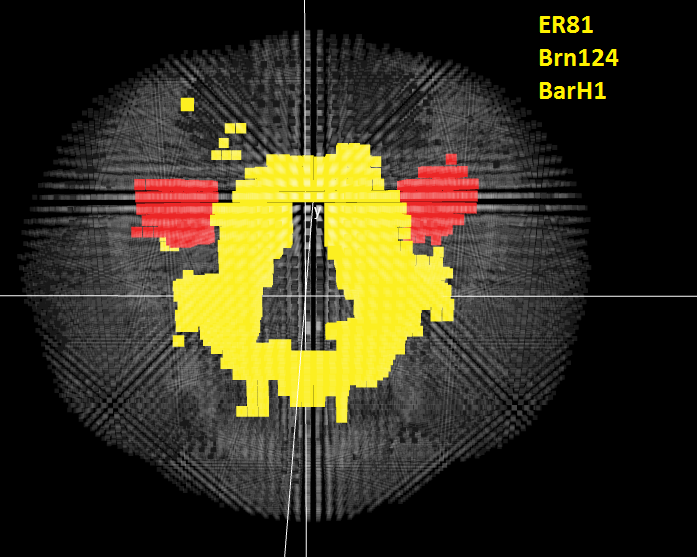
\includegraphics[width=.45\linewidth]{gfx/sup/c21.png}} \quad
        \subfloat[Cluster 22]
        {
        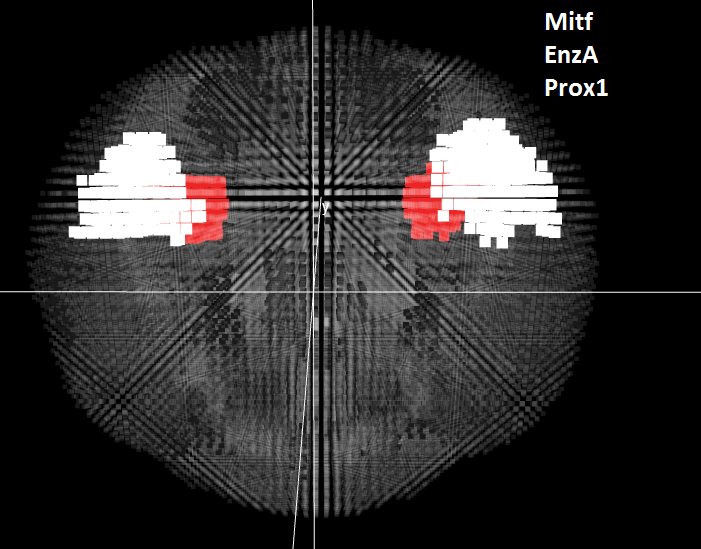
\includegraphics[width=.45\linewidth]{gfx/sup/c22.png}} \\
        \subfloat[Cluster 23]
        {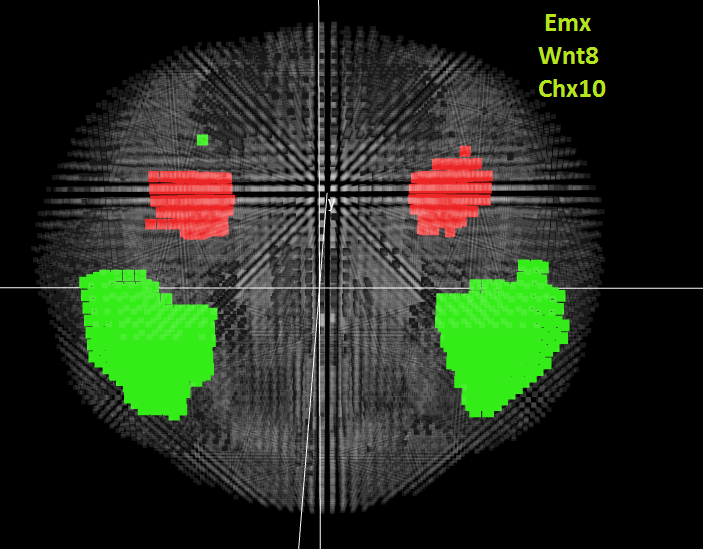
\includegraphics[width=.45\linewidth]{gfx/sup/c23.png}} \quad
        \subfloat[Cluster 24]
        {
        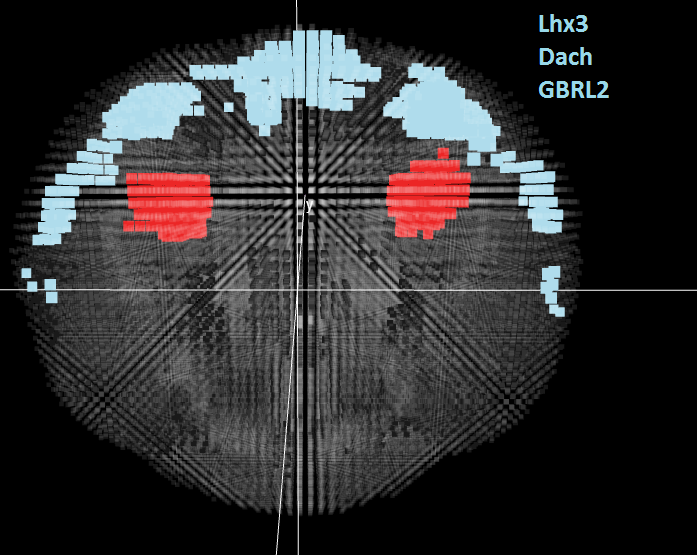
\includegraphics[width=.45\linewidth]{gfx/sup/c24.png}} \\
        \subfloat[Cluster 25]
        {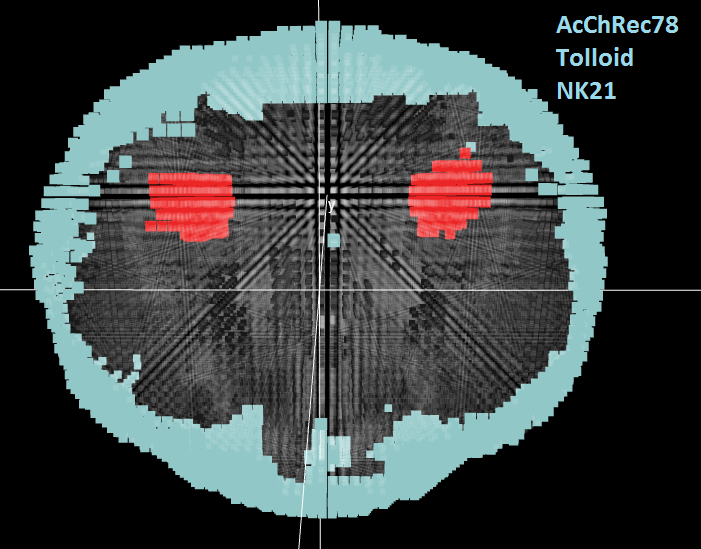
\includegraphics[width=.45\linewidth]{gfx/sup/c25.png}} \quad
        \subfloat[Cluster 26]
        {
        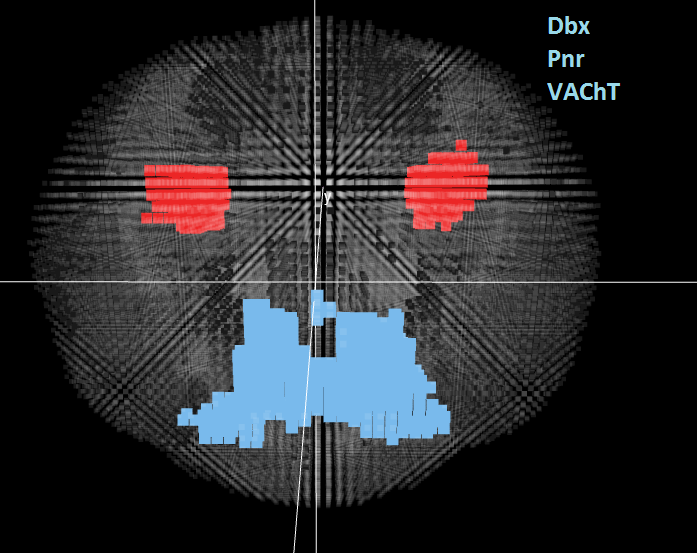
\includegraphics[width=.45\linewidth]{gfx/sup/c26.png}} \\
        \subfloat[Cluster 27]
        {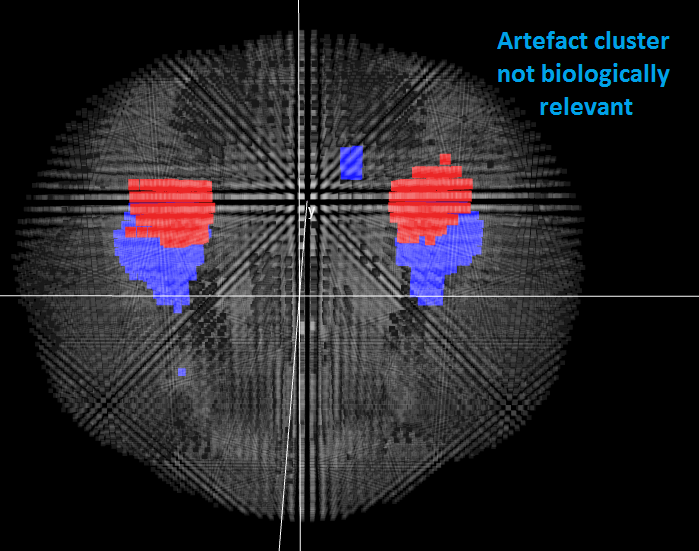
\includegraphics[width=.45\linewidth]{gfx/sup/c27.png}} \quad
        \subfloat[Cluster 28]
        {
        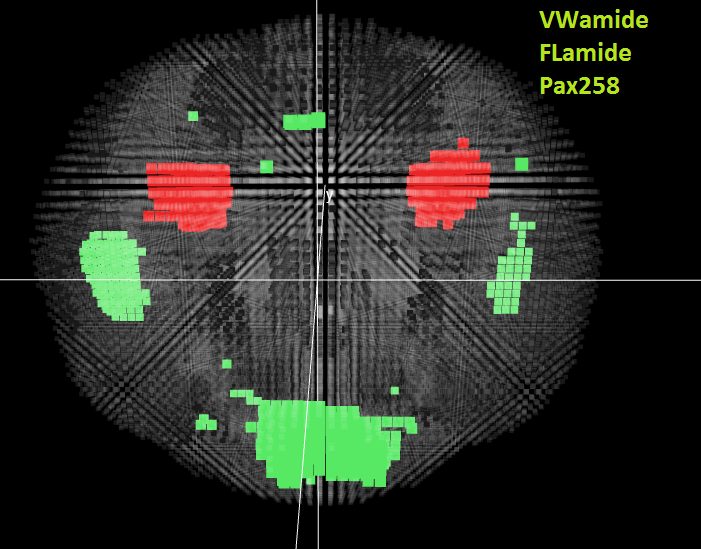
\includegraphics[width=.45\linewidth]{gfx/sup/c28.png}} \\
        \subfloat[Cluster 29]
        {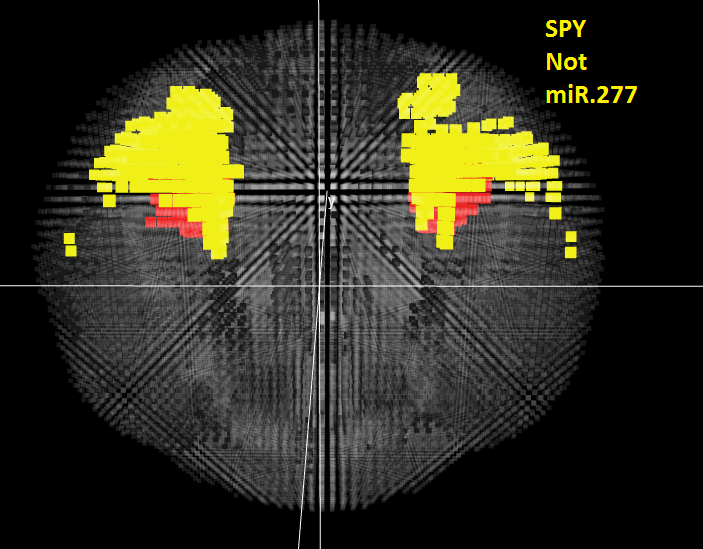
\includegraphics[width=.45\linewidth]{gfx/sup/c29.png}} \quad
        \subfloat[Cluster 30]
        {
        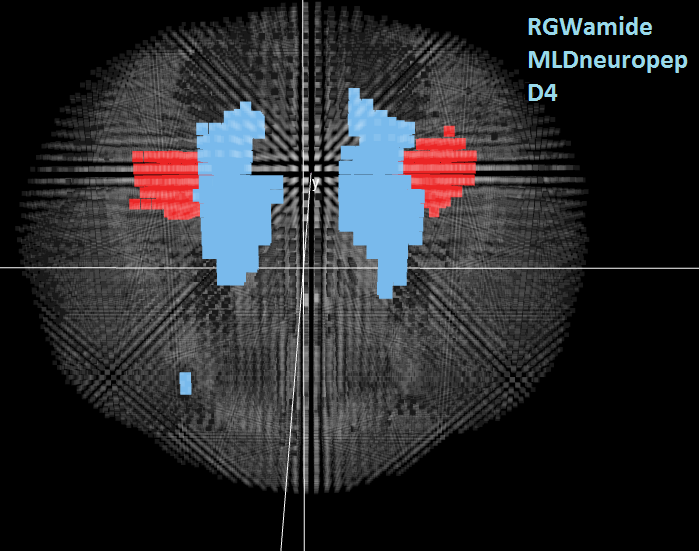
\includegraphics[width=.45\linewidth]{gfx/sup/c30.png}}
\end{figure}

\begin{figure}[bth]
       \ContinuedFloat
        \subfloat[Cluster 31]
        {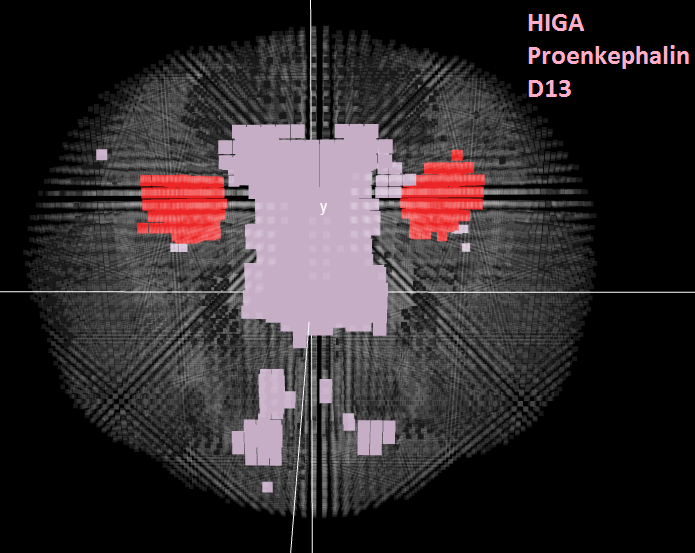
\includegraphics[width=.45\linewidth]{gfx/sup/c31.png}} \quad
        \subfloat[Cluster 32]
        {
        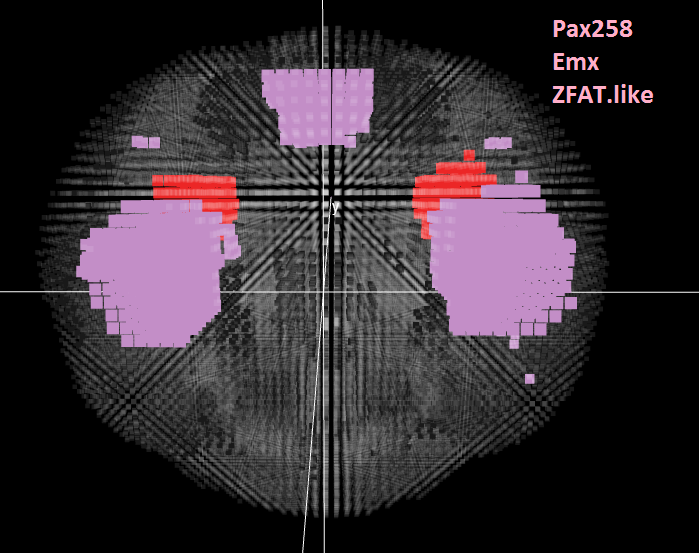
\includegraphics[width=.45\linewidth]{gfx/sup/c32.png}} \\
        \subfloat[Cluster 33]
        {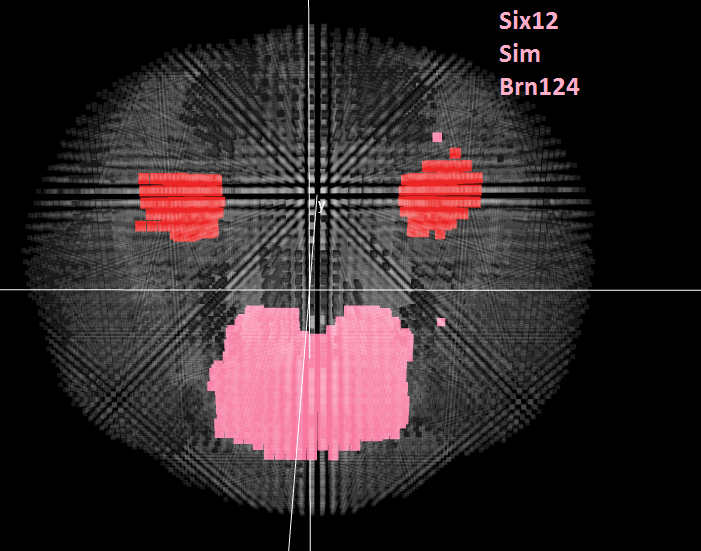
\includegraphics[width=.45\linewidth]{gfx/sup/c33.png}} \quad
        
        
         
        \caption{33 clusters generated by the HMRF method}\label{fig:clusters}
\end{figure}
